
\subsection{RSpecとBDDについて}
ビヘイビア駆動開発(Behaviour-Driven Development : BDD)は,テスト駆動開発(Test-Driven Development : TDD)の工程への理解を深め,それをうまく説明しようとして始まりました.TDDの持つ単語のイメージが構造のテストを中心とするべしというのに対して,BDDはソフトの振る舞いに中心をおきなさいという意図があります.この違いが,初めに考えるべきテストの性質を変化させ,構造ではなく振る舞いを中心にテストを構築するという意識をもたせてくれます.

さらに,ソフトの中で,オブジェクト同士がコミュニケーションをとるように,実世界において開発チームやテストチーム,あるいはドキュメントチーム間のコミュニケーションの取り方をシステムで提供しようというのがBDDのフレームワークです.CucumberとRSpecはこれを実現する一つのシステムとして提供されています.

RSpecとCucumberの関係を図に示しました.これは,RSpec本から書き写した図です[1, pp.9].RSpecでテストを書くと一つ一つのfunctionあるいはmethodレベルでRed, Green, Refactoringを行うべしという意図があります.一方で,もっと大きな枠組み,つまりシステムレベルでもこれらのステップは必要です.ところが,それをRSpecで書くのには無理があります.このレベルのテスト記述をしやすくするのが,Cucumberです.そこでもRed, Green, Refactoringが必要で,そこでサイクルが回ることを意図しています.

\begin{figure}[htbp]\begin{center}
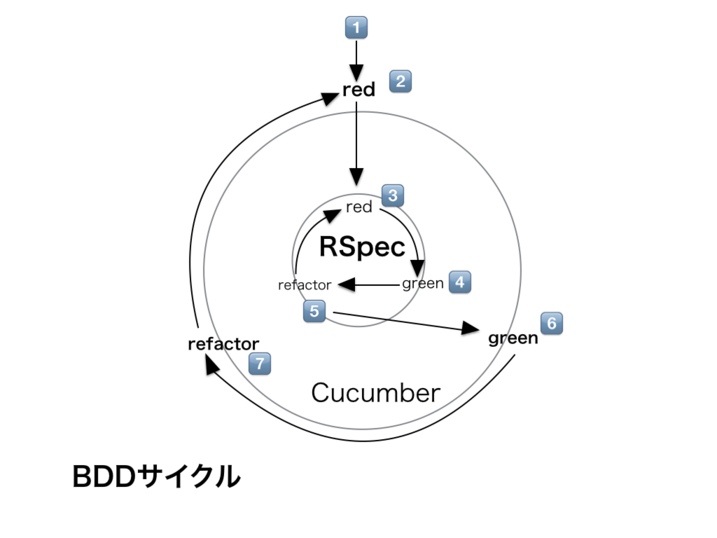
\includegraphics[width=10cm,bb= 0 0 737 553]{../figs/./my_help_nasu.png}
\caption{RSpecとCucumberのRed-Green-Refactoringサイクル間の関係.}
\label{default}\end{center}\end{figure}
BDDの基本的な考え方は次の通りまとめられています.

\begin{quotation}
BDDの目的は,ソフトウェアが使われる状況を説明するための言語を単純化することで,ソフトウェア開発チームのコミュニケーションを後押しすることです.つまり,あるコンテキストで(Given),あるイベントが発生すると(When),ある結果が期待されます(Then).BDDにおけるGiven, When, Thenの3つの単語は,アプリケーションやオブジェクトを,それらの振る舞いに関係なく表現するために使われる単純な単語です.ビジネスアナリスト,テスト担当者,開発者は皆,それらをすぐに理解します.これらの単語はCucumberの言語に直接埋め込まれています[1, pp.3-6].

\end{quotation}
手順を書き直すと次の通りです.

\begin{figure}[htbp]\begin{center}
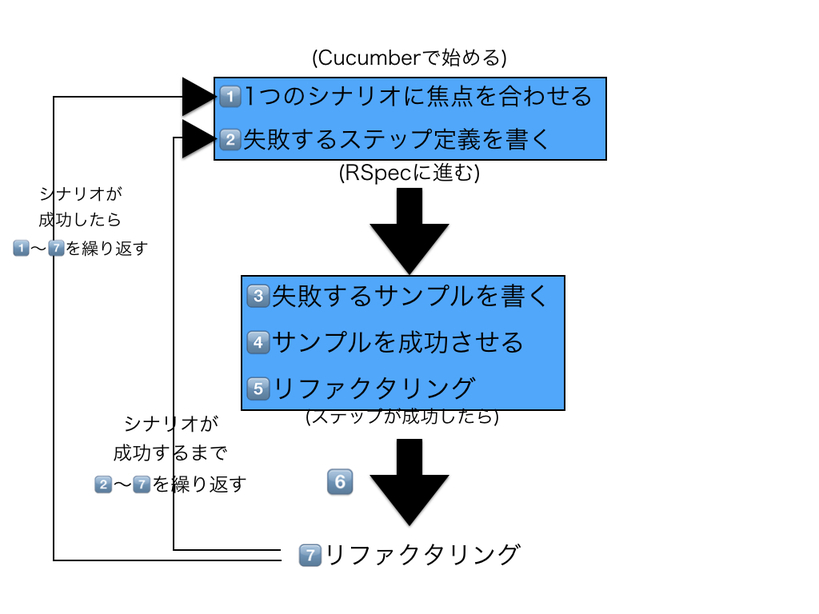
\includegraphics[width=10cm,bb= 0 0 737 553]{../figs/./my_help_nasu1.001.jpg}
\caption{RSpecとCucumberの手順.}
\label{default}\end{center}\end{figure}
まずCucumberで一つのシナリオに焦点を当てて,その振る舞いを記述するfeatureを書きます.一つずつつぶしていくのがこつです.一つのfeatureが書けたら、次に,それぞれfeatureを実現するステップに分けて仕様を決めて行きます.これはTDDのred green refactoringの前に行う作業,「仕様をきめる」に対応しています.このプロセスが終了したら,RSpecに行きます.
RSpecでは実際にテストコードを書き,ここでもred, green, refactoringを行います.
RSpecが成功したら,Cucumberのrefactoringを行います.

